  
\documentclass[english]{article}
\usepackage[T1]{fontenc}
\usepackage[latin9]{inputenc}
\usepackage{float}
\usepackage[a4paper]{geometry}
\usepackage{amsmath}
\DeclareMathOperator*{\argmax}{arg\,max}
\geometry{verbose,tmargin=2cm,bmargin=2cm,lmargin=2cm,rmargin=2cm}
\usepackage{graphicx}
\usepackage{color}

\title{\textbf{CS6700 : Reinforcement Learning } \\ Programming Assignment 1 \\ Report}

\author{Rahul V \\ ME16B171}

\begin{document}

\maketitle

\tableofcontents
\pagebreak
\section{$\epsilon$ - Greedy Algorithm}
\subsection{Implementation}
\begin{itemize}
    \item The estimates of the expected values of rewards for each arm are initialised to zero.
    \item Now, based on the expected values of each arm, an arm is chosen \emph{greedily} 1-$\epsilon$ times and \emph{randomly} $\epsilon$ times from all the available arms.
    \item And after each sample, the expected value of the chosen arm is updated.
    \item As the number of samples increase, the estimates tend to their true values.
\end{itemize}
\subsection{Plots}
\begin{figure}[H]
    \centering
    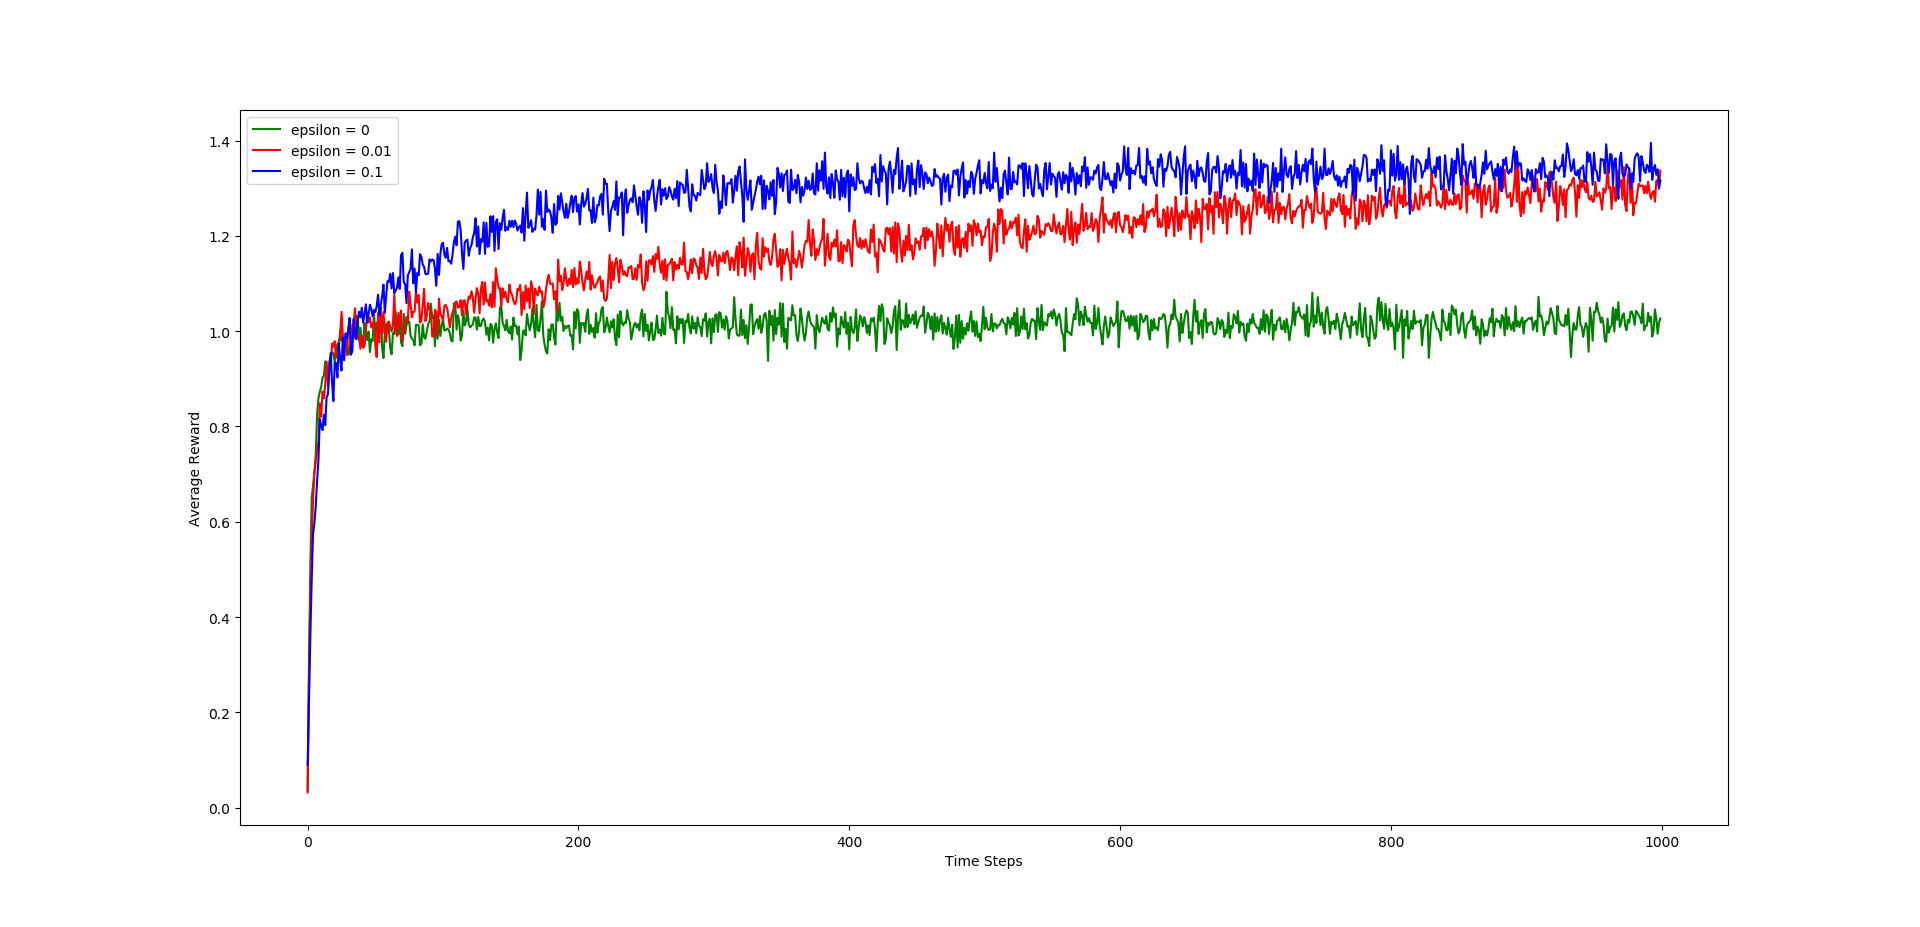
\includegraphics[width=\linewidth]{e_greedy_avg_reward_10arms.png}
    \caption{Plot of average reward of $\epsilon$-greedy algorithm for 10-armed testbed averaged over 2000 runs with different bandits.}
    \label{fig:eg1}
\end{figure}

\begin{figure}[H]
    \centering
    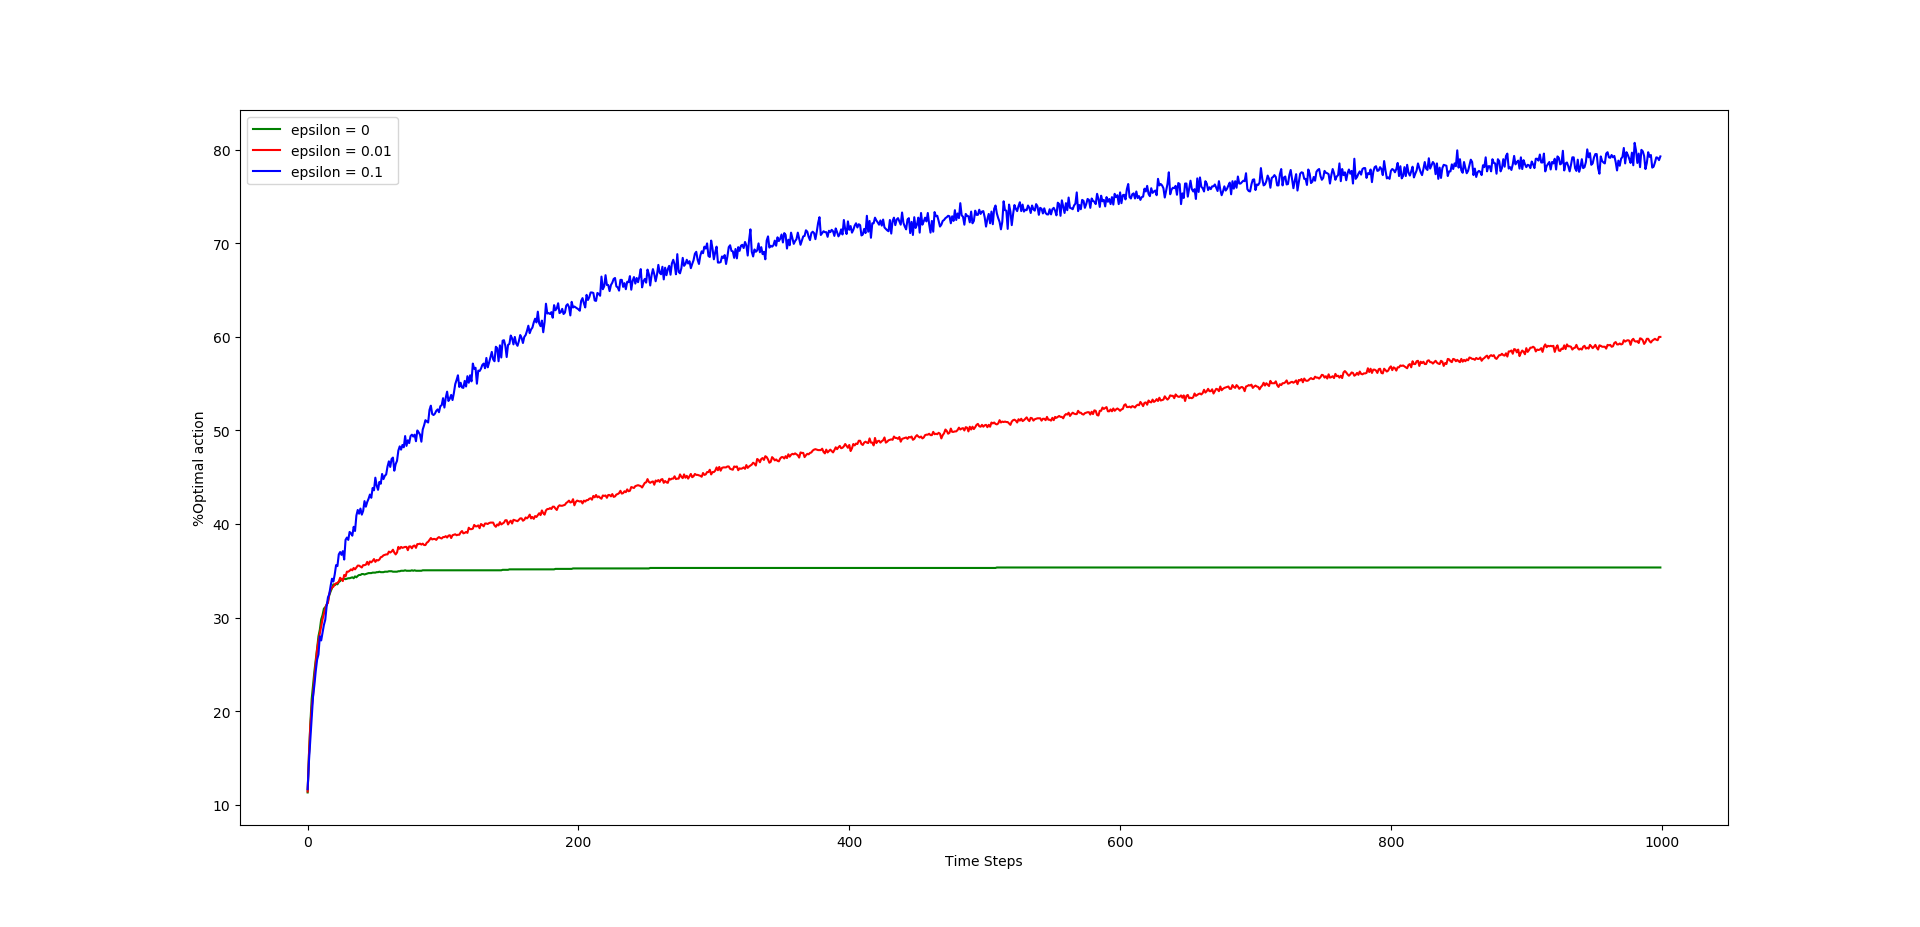
\includegraphics[width=\linewidth]{e_greedy_opt_action_10arms.png}
    \caption{Plot of \% optimal action of $\epsilon$-greedy algorithm for 10-armed testbed averaged over 2000 runs with different bandits.}
    \label{fig:eg1}
\end{figure}

\subsection{Inference}
\begin{itemize}
    \item From the above plots, we can infere that $\epsilon$ = 0.1 perform best both in terms of average reward and \% optimal action.
    \item Whereas the greedy method($\epsilon$ = 0) performs worst in the long run as it picks suboptimal action all the time.
    \item $\epsilon$-greedy method performs better than greedy method as it keeps on exploring other arms and hence has a higher chance of finding the optimal arm.
\end{itemize}
\pagebreak

\section{Softmax Algorithm}
\subsection{Implementaiton}
\begin{itemize}
    \item Softmax algorithm samples arms from Gibbs distribution with temperature as a parameter.
    \item Similar to $\epsilon$-greedy method, the estimates of expected values of arms are initiated to zero and then updated based on the obtained samples from Gibbs distribution.
    \item Probability for picking arm \emph{i} at time \emph{t} is given by  $$ P_{t} = \dfrac{e^{Q_{t}(a_{i})/\tau}}{\sum_{a}e^{Q_{t}(a)/\tau}} $$ where $\tau$ is the temperature parameter.
\end{itemize}

\subsection{Plots}
\begin{figure}[H]
    \centering
    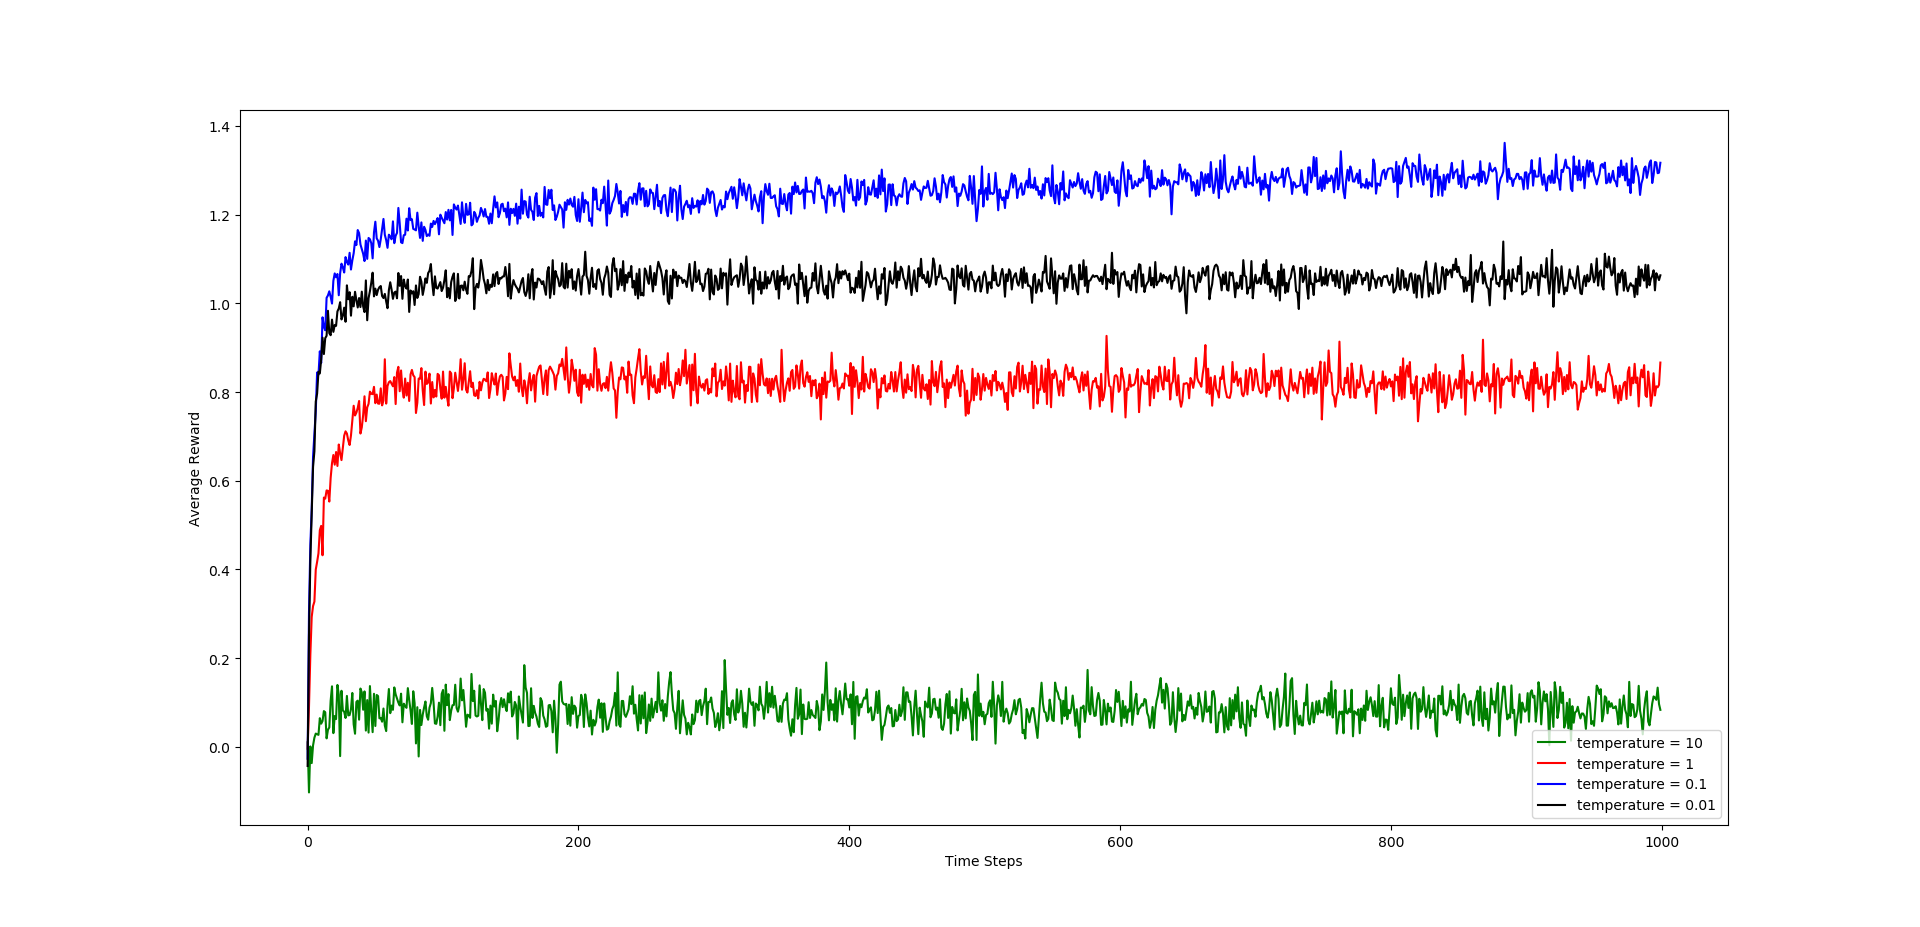
\includegraphics[width=\linewidth]{softmax_avg_reward_10arms.png}
    \caption{Plot of average reward of softmax algorithm for 10-armed testbed averaged over 2000 runs with different bandits.}
    \label{fig:eg1}
\end{figure}

\begin{figure}[H]
    \centering
    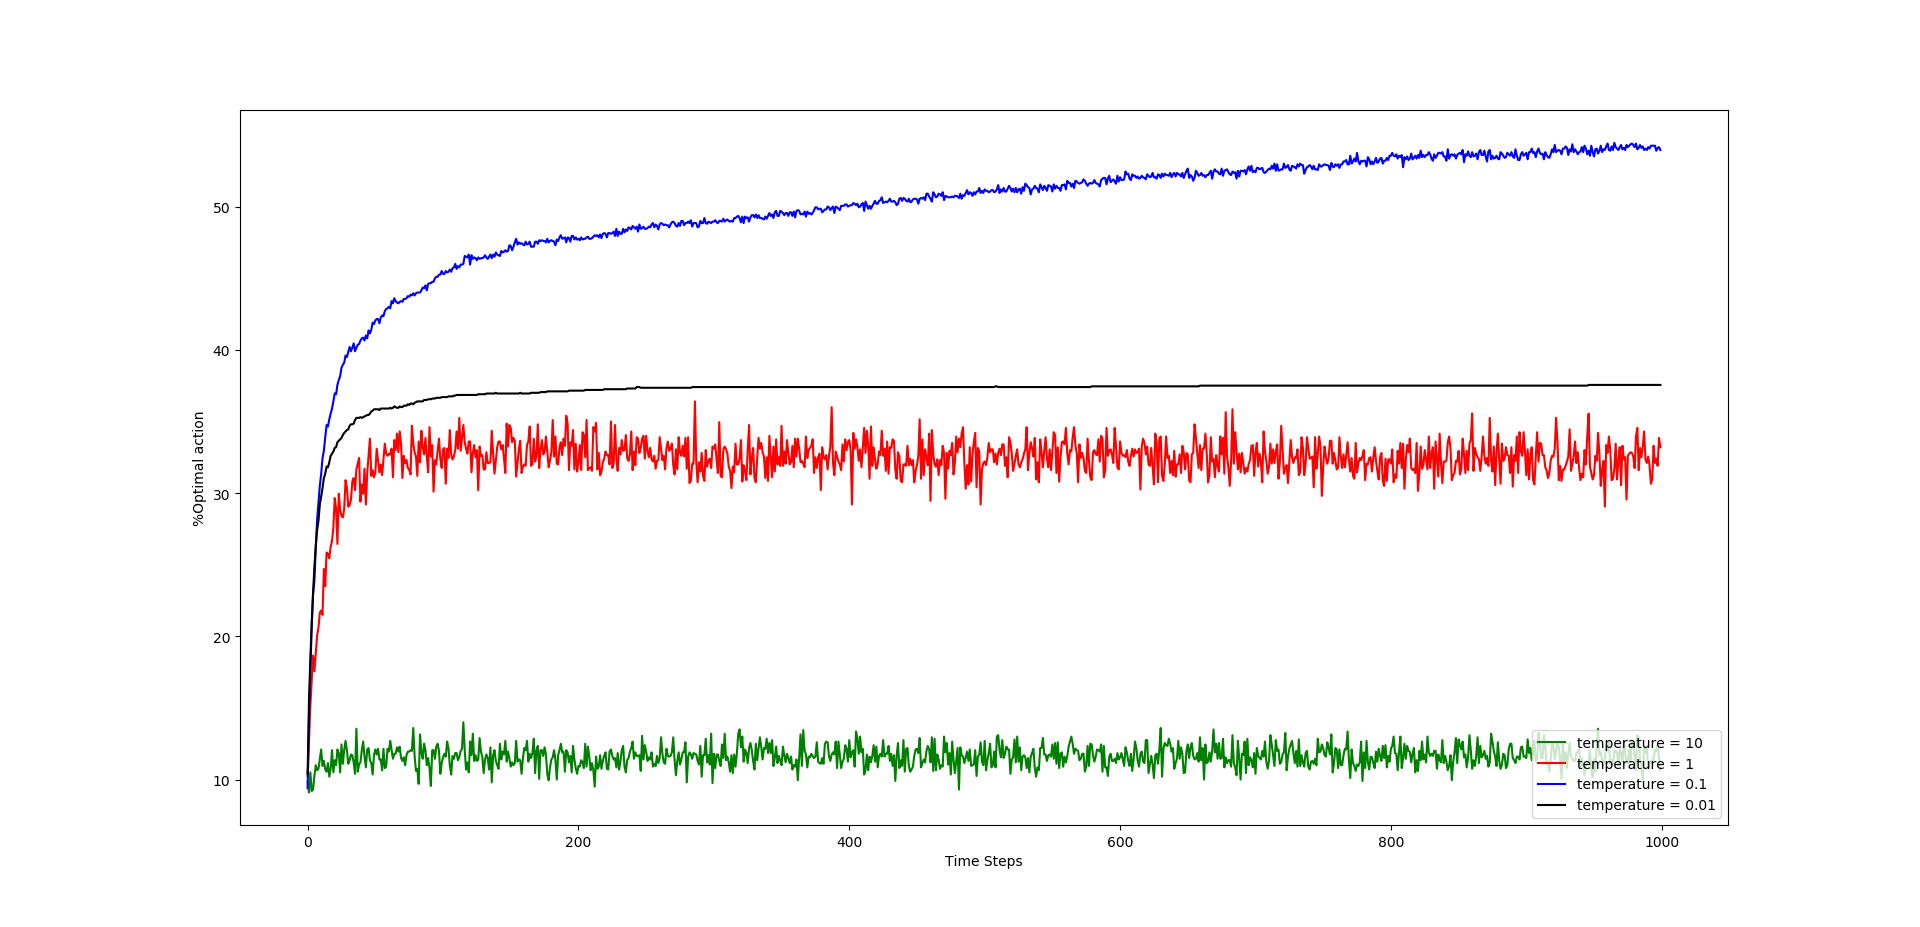
\includegraphics[width=\linewidth]{softmax_opt_action_10arms.png}
    \caption{Plot of \% optimal action of softmax algorithm for 10-armed testbed averaged over 2000 runs with different bandits.}
    \label{fig:eg1}
\end{figure}

\subsection{Inference}
\begin{itemize}
    \item From the above plots, we can infere that for a time step of 1000, temperature of 1000 perform best both in terms of average reward and \% optimal action.
    \item With increase in temperature, the algorithm picks actions more randomly, resulting higher exploration.
    \item With decrease in temperature, the algorith mpicks actions greedily, resulting in exploitation.
    \item At temperature = 0.1, we can find a balance between exploration and exploitation for this bandit. 
\end{itemize}
\pagebreak

\section{UCB1 Algorithm}
\subsection{Implementation}
\begin{itemize}
    \item All the arms are picked atleast once, and then UCB1 algorithm is used to pick the arm with highest upper bound on the estimate of expected value.
    \item The mathematical formula for it is given by $$ a = \argmax_{a} Q(a) + \sqrt{\dfrac{2lnN}{T_{i}(N)}} $$
\end{itemize}
\subsection{Plots}
\begin{figure}[H]
    \centering
    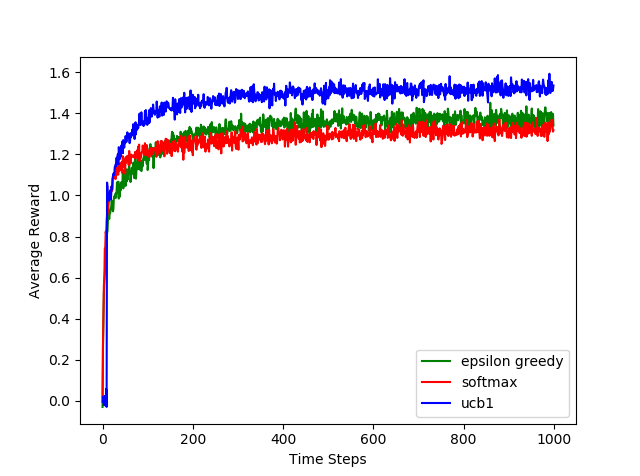
\includegraphics[width=\linewidth]{ucb1_avg_reward_10arms.png}
    \caption{Plot comparing average reward obtained using $\epsilon$-greedy with $\epsilon$ = 0.1, softmax with temperature = 0.1 and UCB1 algorithms for 10-armed testbed averaged over 2000 runs with different bandits.}
    \label{fig:eg1}
\end{figure}

\begin{figure}[H]
    \centering
    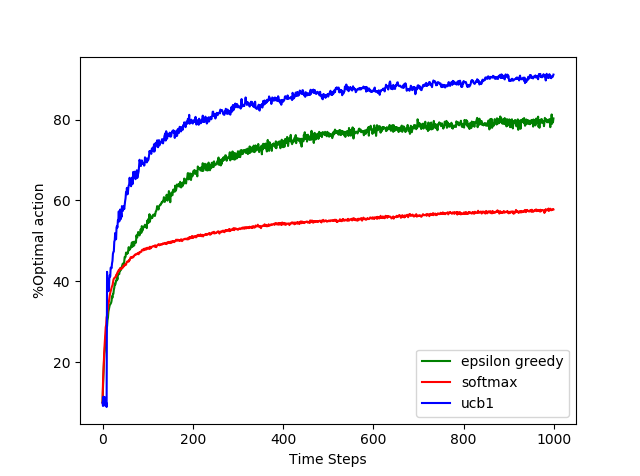
\includegraphics[width=\linewidth]{ucb1_opt_action_10arms.png}
    \caption{Plot of \% optimal actionobtained using $\epsilon$-greedy with $\epsilon$ = 0.1, softmax with temperature = 0.1 and UCB1 algorithms for 10-armed testbed averaged over 2000 runs with different bandits.}
    \label{fig:eg1}
\end{figure}
\subsection{Inference}
\begin{itemize}
    \item From the above plots, we can infere that UCB1 algorithm performs better both in terms of average reward and \% optimal reward when compared to the best performing softmax algorithm and $\epsilon$-greedy algorithm.
    \item This is because UCB1 algorithm explores based on the capability of the arm to out perform the existing greedy arm whereas softmax and $\epsilon$-greedy explore arms with very low estimates too.
\end{itemize}
\pagebreak

\section{Median elimination algorithm}
\subsection{Implementation}
\begin{itemize}
    \item By using $\epsilon$ $\delta$ PAC bounds, we calculate the number of times we should sample each arm.
    \item Then we eliminate the bottom half of the arms based on the estimates we get for the expected values of each arm.
\end{itemize}
\subsection{Plots}
\begin{figure}[H]
    \centering
    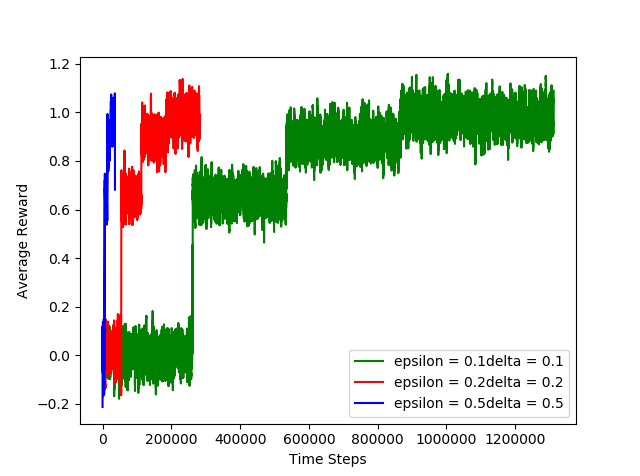
\includegraphics[width=\linewidth]{mea_10arms.png}
    \caption{Plot of average reward for median elimination algorithm for 10-armed testbed after smoothing using savitzy golay filter.}
    \label{fig:eg1}
\end{figure}

\begin{figure}[H]
    \centering
    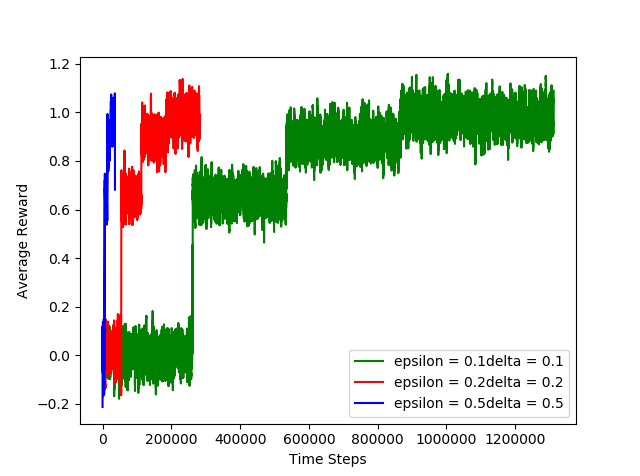
\includegraphics[width=\linewidth]{mea_10arms.png}
    \caption{Plot of \% optimal action for median elimination algorithm for 10-armed testbed after smoothing using savitzy golay filter.}
    \label{fig:eg1}
\end{figure}
\subsection{Inference}
\begin{itemize}
    \item  $\epsilon$ = 0.2 $\delta$ = 0.2 seems to perform better.
    \item The computational cost of computing the median is O(nlogn) where n is the number of arms. This is because for computing median we are essentially sorting the array of estimates of arms and we know that best algorithm for sorting is of O(nlogn).
    \item Yes, it is the rate determining step when the number of arms are not considerably small.
\end{itemize}
\pagebreak

\section{With 1000 Arms}
\subsection{Plots}
\begin{figure}[H]
    \centering
    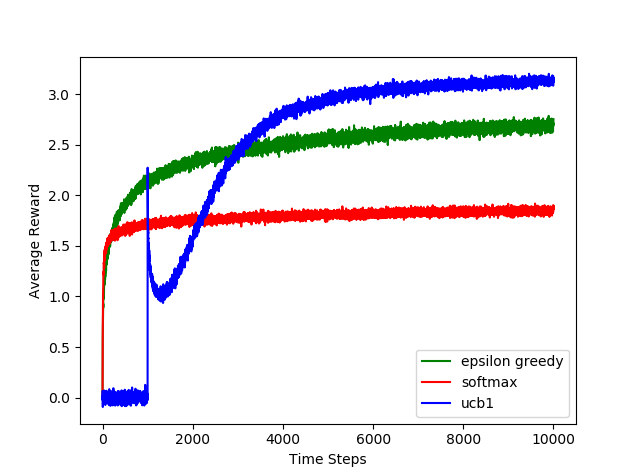
\includegraphics[width=\linewidth]{plot_1000arms_rew.png}
    \caption{Plot comparing average reward obtained using $\epsilon$-greedy with $\epsilon$ = 0.1, softmax with temperature = 0.1 and UCB1 algorithms for 1000-armed testbed averaged over 2000 runs with different bandits.}
    \label{fig:eg1}
\end{figure}

\begin{figure}[H]
    \centering
    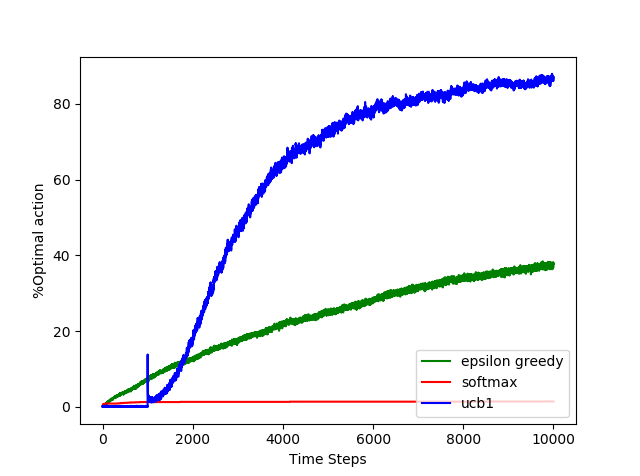
\includegraphics[width=\linewidth]{plot_1000arms_opt.png}
    \caption{Plot of \% optimal action obtained using $\epsilon$-greedy with $\epsilon$ = 0.1, softmax with temperature = 0.1 and UCB1 algorithms for 1000-armed testbed averaged over 2000 runs with different bandits.}
    \label{fig:eg1}
\end{figure}
\subsection{Inference}
\begin{itemize}
    \item As the number of arms grow, UCB1 is still the better algorithm in the long run compared with softmax and $\epsilon$-greedy algorithm for the same above stated reasons.
    \item However intially it takes some time for it try out all the large number of arms. So, it performs worse in the short run.
\end{itemize}
\end{document}